\documentclass{article}
\usepackage[utf8]{inputenc}
\usepackage{amsmath}
\usepackage{graphicx}
\usepackage{hyperref}
\usepackage{fancyhdr}
\usepackage{geometry}
\usepackage{titling}
\usepackage{lipsum}

\geometry{a4paper, margin=2.5cm}

% Header setup
\pagestyle{fancy}
\fancyhf{}
\fancyhead[L]{Projet Optimisation}
\fancyhead[R]{M2 ISD}
\fancyfoot[C]{\thepage}
\renewcommand{\headrulewidth}{0.4pt}
\renewcommand{\footrulewidth}{0pt}

% Remove header on title page but keep footer for page number
\fancypagestyle{plain}{
  \fancyhf{}
  \renewcommand{\headrulewidth}{0pt}
  % Keep footer for page number on title page
}

\title{Projet Vélib: Équilibrage nocturne d’un parc de vélos}
\author{}
\date{}

\begin{document}

% Title page (page de garde)
\begin{titlepage}
    \centering
    \vspace*{4cm}
    {\Huge \bfseries Projet Vélib: Équilibrage nocturne d’un parc de vélos \par}
    \vspace{2cm}
    {\Large \textbf{Nom :} Nazim KESKES \par}
    \vspace{0.5cm}
    {\Large \textbf{Module :} Optimisation \par}
    \vspace{0.5cm}
    {\Large \textbf{Formation :} Master 2 ISD \par}
    \vspace{0.5cm}
    {\Large \textbf{Année scolaire :} 2024-2025 \par}
    \vfill
\end{titlepage}

\setcounter{page}{1}
\pagenumbering{roman}
\tableofcontents
\newpage
\pagenumbering{arabic}

\maketitle

\section{Introduction}
Ce projet porte sur l'optimisation de la gestion d'un parc de vélos en libre-service dans une grande ville. L'objectif principal est de modéliser et résoudre un problème lié à l'équilibrage nocturne des stations de vélos. Ce problème est crucial pour assurer une distribution équitable des vélos entre les stations, minimisant ainsi les déséquilibres qui peuvent causer des insatisfactions chez les utilisateurs.

\section{Description du Problème}
Une entreprise gère un parc de vélos en libre-service avec de nombreuses stations réparties dans une grande ville. Les stations sont plus ou moins attractives, ce qui entraîne des fluctuations importantes du nombre de vélos disponibles au cours de la journée. Ce déséquilibre pose deux problèmes principaux :
\begin{enumerate}
    \item Les stations peu attractives peuvent manquer de vélos, frustrant les utilisateurs qui ne trouvent pas de vélos disponibles.
    \item Les stations très attractives peuvent être saturées, obligeant les utilisateurs à se rendre à d'autres stations pour déposer leur vélo.
\end{enumerate}
Pour pallier ces inconvénients, l'entreprise effectue des opérations d'équilibrage nocturne : un semi-remorque circule entre les stations pour désengorger les stations saturées et déposer des vélos dans celles qui en manquent.
Le but de ce projet est la prévision de la tournée du semi-remorque qui équilibre les stations de vélos. La tournée commence au magasin, où est gardé un stock suffisamment grand de vélos. On charge au magasin le semi-remorque avec un certain nombre de vélos, ce nombre fait partie des inconnues du problème. Puis le semi-remorque doit passer par chacune des $n$ stations qui composent le parc, y compris par les stations déjà équilibrées. La tournée se termine par le retour du semi-remorque au magasin, pas nécessairement à vide. Chaque station n’est visitée qu’une unique fois et la capacité du semi-remorque doit être respectée.
Les données du problème incluent :
\begin{itemize}
    \item Le nombre $n$ de stations concernées par la tournée et leur emplacement géographique
    \item La capacité $K$ du semi-remorque
    \item La distance entre deux stations $i$ et $j$ ainsi que la distance du magasin à chacune des stations
    \item Le nombre de vélos effectivement présents à la station $i$ ainsi que la capacité maximale de la station $i$
    \item Le nombre idéal de vélos qui doivent se trouver à la station $i$ pour permettre un bon fonctionnement de la station
\end{itemize}
Les objectifs visés pour la tournée sont :
\begin{enumerate}
    \item Savoir si, connaissant les données du problème, il est possible de remettre chaque station à son niveau idéal de vélos en une unique tournée
    \item Parmi l’ensemble des tournées possibles qui minimise le déséquilibre global, laquelle permet de parcourir la plus petite distance globale
\end{enumerate}
Un premier objectif consiste donc à organiser la tournée de sorte à minimiser (et si possible annuler) le déséquilibre global, défini comme la somme des déséquilibres de chaque station. Un second objectif, moins prioritaire que le premier, consiste à minimiser la distance totale parcourue après avoir minimisé le déséquilibre, pour des raisons évidentes d’efficacité et d’économie d’énergie.
\section{Modélisation du Problème}
La modélisation du problème proposée dans ce rapport est basée sur une approche quadratique en variables 0-1 et entières. Voici les éléments clés de cette modélisation :

\subsection{Données d'Entrée}
\begin{itemize}
    \item $n$ : nombre de stations
    \item $K$ : capacité du camion
    \item $nbvp_i$ : vélos présents initialement à la station $i$
    \item $cap_i$ : capacité de la station $i$
    \item $ideal_i$ : nombre idéal de vélos pour la station $i$
    \item $d_{ik}$ : distance entre stations $i$ et $k$ (arrondie à l'entier le plus proche)
\end{itemize}

\subsection{Variables de Décision}
\begin{itemize}
    \item $x_{ij}$ : variable binaire valant 1 si la station $i$ est visitée en position $j$
    \item $charge_j$ : nombre de vélos dans le camion après la $j$-ème étape
    \item $depot_{ij}$ : nombre de vélos déposés ou retirés à la station $i$ à l'étape $j$
\end{itemize}

\subsection{Variables Auxiliaires}
\begin{itemize}
    \item $d_i^+$ : excédent par rapport à l'idéal
    \item $d_i^-$ : déficit par rapport à l'idéal
    \item $y_{ijk}$ : produit $x_{ij} \times x_{k,j+1}$ pour linéarisation
\end{itemize}

\subsection{Contraintes Détaillées}
\subsubsection{Contraintes de Routage}
\[
\begin{cases}
\sum_{j=1}^n x_{ij} = 1 & \forall i \in \{1,...,n\} \\
\sum_{i=1}^n x_{ij} = 1 & \forall j \in \{1,...,n\} \\
x_{ij} \in \{0,1\} & \forall i,j
\end{cases}
\]

\subsubsection{Contraintes de Flux}
\[
charge_j = charge_{j-1} - \sum_{i=1}^n depot_{ij} \cdot x_{ij} \quad \forall j \in \{1,...,n\}
\]

\subsubsection{Contraintes de Capacité}
\[
\begin{cases}
0 \leq charge_j \leq K & \forall j \\
nbvp_i + \sum_{j=1}^n depot_{ij} \leq cap_i & \forall i \\
\sum_{j=1}^n depot_{ij} \geq -nbvp_i & \forall i
\end{cases}
\]

\subsection{Fonction Objective du problème (Approche Lexicographique)}
\subsubsection{Premier Niveau : Minimiser le Déséquilibre Global}
\[
\min \quad d^* = \sum_{i=1}^n (d_i^+ + d_i^-)
\]

\subsubsection{Deuxième Niveau : Minimiser la Distance parmi les solutions optimales}
\[
\min \quad D = \sum_{j=1}^{n-1} \sum_{i=1}^n \sum_{k=1}^n x_{ij} x_{k,j+1} d_{ik} + \sum_{i=1}^n x_{i1} d_{0i} + \sum_{i=1}^n x_{in} d_{i0}
\]

sous la contrainte additionnelle :
\[
\sum_{i=1}^n (d_i^+ + d_i^-) = d^*
\]

où $d^*$ est la valeur optimale obtenue au premier niveau.

\subsection{Linéarisation du Problème}
\subsubsection{Variables de Linéarisation}
Les variables $y_{ijk}$ remplacent les produits $x_{ij}x_{k,j+1}$ dans le calcul de la distance totale.

\subsubsection{Substitution des Termes Quadratiques}
Pour chaque triplet $(i,j,k)$ avec $j \in \{1,...,n-1\}$ :
\[
\begin{cases}
y_{ijk} \leq x_{ij} \\
y_{ijk} \leq x_{k,j+1} \\
y_{ijk} \geq x_{ij} + x_{k,j+1} - 1 \\
y_{ijk} \geq 0
\end{cases}
\]

\subsubsection{Formulation Linéaire pour l'Approche Lexicographique}
\paragraph{Première Étape (Déséquilibre) :}
\[
\min \sum_i (d_i^+ + d_i^-)
\]

\paragraph{Deuxième Étape (Distance) :}
\[
\min \left[\sum_{i,k,j} y_{ijk} d_{ik} + \sum_i (x_{i1} d_{0i} + x_{in} d_{i0})\right]
\]

sous la contrainte :
\[
\sum_i (d_i^+ + d_i^-) = d^*
\]

\section{Résolution du Problème}

Pour résoudre le problème d'équilibrage des stations de vélos, nous avons implémenté deux méthodes distinctes : la méta-heuristique du recuit simulé et une heuristique originale de balancement progressif par zones.

\subsection{Recuit Simulé}

Le recuit simulé est une méthode d'optimisation inspirée du processus de recuit en métallurgie. Cette approche permet d'explorer l'espace des solutions en acceptant initialement des solutions moins optimales pour éviter les minima locaux. La température diminue progressivement, réduisant la probabilité d'accepter des solutions moins bonnes au fil du temps.

Notre implémentation du recuit simulé pour ce problème suit une approche lexicographique en deux phases :

\begin{enumerate}
\item \textbf{Phase 1 : Minimisation du déséquilibre global}

  La fonction objectif pour cette phase est :
  \[
  \min \quad d^* = \sum_{i=1}^n (d_i^+ + d_i^-)
  \]
  où $d_i^+$ représente l'excédent par rapport à l'idéal et $d_i^-$ représente le déficit par rapport à l'idéal pour la station $i$.

  \begin{itemize}
    \item L'algorithme commence par une solution initiale aléatoire.
    \item À chaque itération, deux stations sont échangées de manière aléatoire.
    \item La nouvelle solution est acceptée si elle améliore le déséquilibre ou selon une probabilité basée sur la température actuelle.
    \item La température diminue progressivement selon un taux de refroidissement adaptatif.
    \item Cette phase se termine lorsque la température devient très faible ou après un nombre maximal d'itérations.
  \end{itemize}

\item \textbf{Phase 2 : Minimisation de la distance}

  La fonction objectif pour cette phase est :
  \[
  \min \quad D = \sum_{j=1}^{n-1} \sum_{i=1}^n \sum_{k=1}^n x_{ij} x_{k,j+1} d_{ik} + \sum_{i=1}^n x_{i1} d_{0i} + \sum_{i=1}^n x_{in} d_{i0}
  \]
  sous la contrainte :
  \[
  \sum_{i=1}^n (d_i^+ + d_i^-) = d^*
  \]
  où $d^*$ est la valeur optimale obtenue au premier niveau.

  \begin{itemize}
    \item En partant de la meilleure solution de la phase 1, l'algorithme cherche à minimiser la distance totale parcourue tout en maintenant le déséquilibre optimal.
    \item Le processus est similaire à la phase 1, mais la fonction de coût prend en compte la distance parcourue uniquement pour les solutions ayant le déséquilibre optimal.
  \end{itemize}
\end{enumerate}

\subsubsection{Notion de Voisinage}

Dans le contexte du recuit simulé, la notion de voisinage est cruciale. Pour notre problème, nous avons défini le voisinage comme l'ensemble des solutions obtenues en échangeant deux stations dans la tournée actuelle. Cette définition permet d'explorer efficacement l'espace des solutions tout en restant proche de la solution courante, favorisant ainsi des améliorations incrémentales. En d'autres termes, à chaque itération, nous générons de nouvelles solutions en échangeant deux stations de la tournée actuelle, ce qui permet d'explorer des solutions voisines qui pourraient potentiellement améliorer la solution courante.

\subsubsection{Modèles Adaptés pour les Bornes Inférieures}

Pour déterminer les bornes inférieures du déséquilibre et de la distance, nous avons adapté le modèle initial en nombres entiers de la manière suivante :

\begin{enumerate}
\item \textbf{Déséquilibre} : La borne inférieure du déséquilibre est calculée comme la somme des déséquilibres individuels de chaque station. Le déséquilibre d'une station est défini comme la différence absolue entre le nombre idéal de vélos et le nombre actuel de vélos. Mathématiquement, cela peut être exprimé comme :
  \[
  \text{Borne inférieure du déséquilibre} = \sum_{i=1}^n |ideal_i - nbp_i|
  \]
  où $ideal_i$ est le nombre idéal de vélos pour la station $i$ et $nbp_i$ est le nombre actuel de vélos à la station $i$.

\item \textbf{Distance} : La borne inférieure de la distance est calculée en utilisant le problème du voyageur de commerce (TSP) sur les stations à visiter. Nous avons adapté le modèle pour inclure les contraintes spécifiques de notre problème, notamment la capacité du semi-remorque et les opérations de dépôt/retrait de vélos. Mathématiquement, cela peut être exprimé comme :
  \[
  \text{Borne inférieure de la distance} = \min \sum_{i=1}^n \sum_{j=1}^n d_{ij} x_{ij}
  \]
  sous les contraintes :
  \[
  \sum_{j=1}^n x_{ij} = 1 \quad \forall i
  \]
  \[
  \sum_{i=1}^n x_{ij} = 1 \quad \forall j
  \]
  \[
  x_{ij} \in \{0,1\} \quad \forall i,j
  \]
  où $d_{ij}$ est la distance entre les stations $i$ et $j$, et $x_{ij}$ est une variable binaire indiquant si la station $j$ est visitée immédiatement après la station $i$.
\end{enumerate}

\subsubsection{Résultats de la méthode de recuit simulé}

Dans cette section, nous présentons les résultats obtenus avec la méthode de recuit simulé lexicographique pour différentes instances du problème. Pour chaque instance, le tableau présente le nombre de stations $N$, la capacité du semi-remorque $K$, le déséquilibre minimal $d^*$, la distance minimale $D^*$, ainsi que le temps d'exécution en secondes.

Les résultats obtenus avec la méthode de recuit simulé lexicographique sont résumés dans le tableau \ref{tab:resultats_recuit}. Pour chaque instance, le tableau présente le nombre de stations $N$, la capacité du semi-remorque $K$, le déséquilibre minimal $d^*$, la distance minimale $D^*$, ainsi que le temps d'exécution en secondes.

\begin{table}[h!]
\centering
\begin{tabular}{|c|c|c|c|c|c|}
\hline
Instance & $N$ & $K$ & $d^*$ & $D^*$ & Temps (s) \\
\hline
Instance 1 & 10 & 6 & 1.00 & 447.00 & 17.99 \\
Instance 2 & 20 & 11 & 6.00 & 409.00 & 86.08 \\
Instance 3 & 20 & 11 & 15.00 & 413.00 & 97.18 \\
Instance 4 & 50 & 10 & 6.00 & 831.00 & 492.53 \\
Instance 5 & 100 & 10 & 20.00 & 1039.00 & 1410.38 \\
Instance 6 & 200 & 10 & 80.00 & 1367.00 & 4246.41 \\
Instance 7 & 200 & 14 & 71.00 & 1382.00 & 4287.81 \\
Instance 8 & 200 & 12 & 85.00 & 1599.00 & 11482.35 \\
Instance 9 & 500 & 14 & 291.00 & 10185.00 & 11482.35 \\
\hline
\end{tabular}

\vspace{0.5cm}
\caption{Tableau présentant les résultats de la méthode de recuit simulé lexicographique pour différentes instances du problème.}
\end{table}

\subsubsection{Paramètres et formule de refroidissement}

La méthode de recuit simulé lexicographique utilise deux phases avec des paramètres fixés dans le code source :

\begin{itemize}
  \item \textbf{Température initiale} ($T_0$) : Fixée à 1000.0.

  \item \textbf{Seuil de température minimale} ($T_{\min}$) : Un seuil de $3 \times 10^{-2}$ est utilisé pour arrêter le processus de refroidissement avant d'atteindre le nombre maximal d'itérations.

  \item \textbf{Nombre maximum d'itérations} : $10^7$ pour la phase 1 (minimisation du déséquilibre) et $10^8$ pour la phase 2 (minimisation de la distance).

  \item \textbf{Refroidissement} ($R$) : Le taux de refroidissement adaptatif est calculé selon la formule
  \[
  R = \exp\left(\log(1 - 5 \times 10^{-6}) \times \frac{K_0 \times N_0}{K \times N}\right)
  \]
  où $K_0$ et $N_0$ correspondent respectivement à la capacité et au nombre de stations de la première instance testée. Cette approche permet d'affiner la formule adaptative pour les instances de plus grande taille, qui nécessitent un refroidissement plus lent afin d'assurer une meilleure précision en fin d'optimisation.
\end{itemize}

Après plusieurs expérimentations, nous avons remarqué que les instances avec des valeurs relativement petites de $(K, N)$ nécessitent un taux de refroidissement compris entre $10^{-5}$ et $10^{-6}$ pour atteindre le résultat optimal sans forcément atteindre le maximum d'itérations. En revanche, les instances avec des valeurs plus grandes de $(K, N)$ requièrent plus d'itérations et de temps pour converger vers un résultat proche de l'optimal. C'est pourquoi nous avons proposé un refroidissement adaptatif qui, en fonction de la grandeur de $(K, N)$ et avec des valeurs de référence $K_0$ et $N_0$ (correspondant dans cet exemple à la capacité et au nombre de stations de la première instance), permet d'ajuster le taux de refroidissement pour offrir plus d'itérations aux grandes instances, assurant ainsi une meilleure précision.



\subsection{Heuristique de Balancement Progressif par Zones}

Cette heuristique a été proposée par moi-même et est inspirée des techniques de clustering adaptatif, de l’algorithme des économies de Clarke et Wright et de l’optimisation lexicographique en deux phases.

\begin{enumerate}
  \item \textbf{Division de l'espace en zones}
    \begin{itemize}
      \item L'algorithme commence par créer des zones adaptatives basées sur la densité de déséquilibre et la proximité géographique.
      \item Les stations avec le plus grand déséquilibre deviennent les centres initiaux des zones.
      \item Les stations restantes sont assignées à la zone la plus appropriée en fonction de la distance et de la compatibilité de déséquilibre.
    \end{itemize}

  \item \textbf{Traitement des zones par ordre de priorité}
    \begin{itemize}
      \item Les zones sont triées par priorité décroissante, celles avec le plus grand déséquilibre total étant traitées en premier.
      \item Pour chaque zone, l'ordre de visite des stations est optimisé localement en utilisant plusieurs stratégies :
        \begin{itemize}
          \item Plus proche voisin avec prise en compte du déséquilibre
          \item Algorithme des économies adapté pour une zone
          \item Optimisation 2-opt pour améliorer la route
        \end{itemize}
    \end{itemize}

  \item \textbf{Stratégie de réajustement adaptatif entre les zones}
    \begin{itemize}
      \item Après avoir traité toutes les zones, l'algorithme applique des améliorations locales par échanges adaptatifs.
      \item Ces améliorations se font en trois phases :
        \begin{itemize}
          \item Échanges locaux entre stations adjacentes
          \item Échanges inter-zones pour améliorer la transition entre zones
          \item Réorganisation de segments de la route pour réduire la distance totale
        \end{itemize}
    \end{itemize}

  \item \textbf{Optimisation Lexicographique}
    \begin{itemize}
      \item Première étape : minimiser le déséquilibre global.
      \item Deuxième étape : minimiser la distance totale parmi les solutions ayant le déséquilibre optimal.
    \end{itemize}
\end{enumerate}

Cette méthode permet d'obtenir des solutions de bonne qualité tout en étant plus rapide que le recuit simulé pour les grandes instances.

\subsubsection{Notion de Voisinage}
Pour l’heuristique de zones progressives, le voisinage est défini par trois types de mouvements simples :
\begin{itemize}
  \item \textbf{Échanges locaux} : permutation de deux stations adjacentes dans la tournée.
  \item \textbf{Échanges inter-zones} : permutation de deux stations appartenant à des zones différentes.
  \item \textbf{Réorganisation de segments} : extraction et permutation d’un petit segment de la tournée.
\end{itemize}
Ces opérations permettent d’explorer efficacement des solutions voisines et de réaliser des améliorations incrémentales tout au long de l’optimisation.

\subsubsection{Modèles Adaptés pour les Bornes Inférieures}
Pour estimer les bornes inférieures du problème de balancement progressif par zones, on utilise :
\begin{itemize}
  \item \textbf{Borne du déséquilibre} : somme des déséquilibres individuels
  \[\sum_{i=1}^n |ideal_i - nbp_i|\].
  \item \textbf{Borne de la distance} : solution relaxée du TSP sur l’ensemble des stations, sans prendre en compte la capacité du camion ni les opérations de dépôt/retrait.
\end{itemize}

\subsubsection{Résultats Obtenus}

Dans cette section, nous présentons les résultats obtenus par notre heuristique de balancement progressif par zones pour différentes instances du problème. Les instances varient en termes de nombre de stations ($N$) et de capacité du semi-remorque ($K$). Pour chaque instance, nous rapportons le déséquilibre minimal atteint ($d^*$), la distance minimale parcourue ($D^*$), ainsi que le temps d'exécution en secondes.
\begin{table}[!h]
    \centering
    \begin{tabular}{|c|c|c|c|c|c|}
        \hline
        Instance & $N$ & $K$ & $d^*$ & $D^*$ & Temps (s) \\
        \hline
        Instance 1 & 10 & 6 & 1.00 & 481.00 & 2.05 \\
        Instance 2 & 20 & 11 & 6.00 & 427.00 & 3.46 \\
        Instance 3 & 20 & 11 & 15.00 & 428.00 & 3.71 \\
        Instance 4 & 50 & 10 & 6.00 & 772.00 & 67.30 \\
        Instance 5 & 100 & 10 & 8.00 & 1094.00 & 545.72 \\
        Instance 6 & 200 & 10 & 0.00 & 1955.00 & 3948.20 \\
        Instance 7 & 200 & 14 & 7.00 & 1697.00 & 4294.98 \\
        Instance 8 & 200 & 12 & 69.00 & 1528.00 & 4354.01 \\
        Instance 9 & 500 & 14 & 85.00 & 3824.00 & 9675.67 \\
        \hline
    \end{tabular}
    \caption{Résultats de l'heuristique de balancement progressif par zones}
\end{table}
       \section{Comparaison des Méthodes}
       
       Dans cette section, nous comparons les deux méthodes proposées pour résoudre le problème d'équilibrage nocturne des stations de vélos : la méthode de recuit simulé et l'heuristique de balancement progressif par zones. La comparaison porte sur trois métriques principales : le temps d'exécution, la distance totale parcourue, et le déséquilibre global.
       
       \subsection{Analyse des Métriques}
       
       \begin{itemize}
           \item \textbf{Temps d'exécution :} La méthode de recuit simulé est significativement plus lente que l'heuristique de balancement progressif, surtout pour les grandes instances. Par exemple, pour l'instance 9, le recuit simulé prend environ 11482 secondes, tandis que l'heuristique s'exécute en moins de 10000 secondes. Cette différence s'explique par la nature itérative et exhaustive du recuit simulé, comparée à l'approche plus ciblée et locale de l'heuristique.
\end{itemize}

\begin{figure}[htbp]
    \centering
    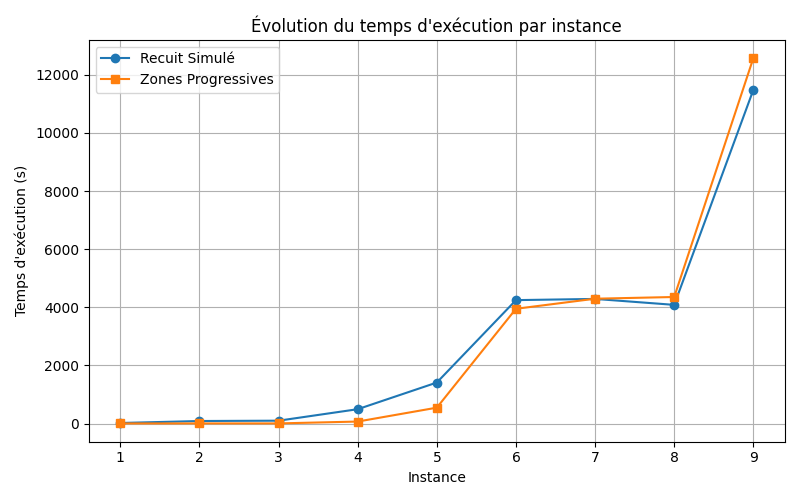
\includegraphics[width=0.7\textwidth]{temps.png}
    \caption{Comparaison des temps d'exécution entre les deux méthodes}
\end{figure}

\begin{itemize}
    \item \textbf{Distance parcourue :} En général, la méthode de recuit simulé tend à minimiser la distance totale parcourue plus efficacement que l'heuristique, notamment pour les grandes instances. Par exemple, pour l'instance 9, la distance minimale obtenue par le recuit est de 10185, contre 3824 pour l'heuristique. Cependant, il est important de noter que pour certaines instances, l'heuristique peut produire des distances plus élevées, ce qui peut être un compromis acceptable compte tenu du gain en temps d'exécution.
\end{itemize}

\begin{figure}[htbp]
    \centering
    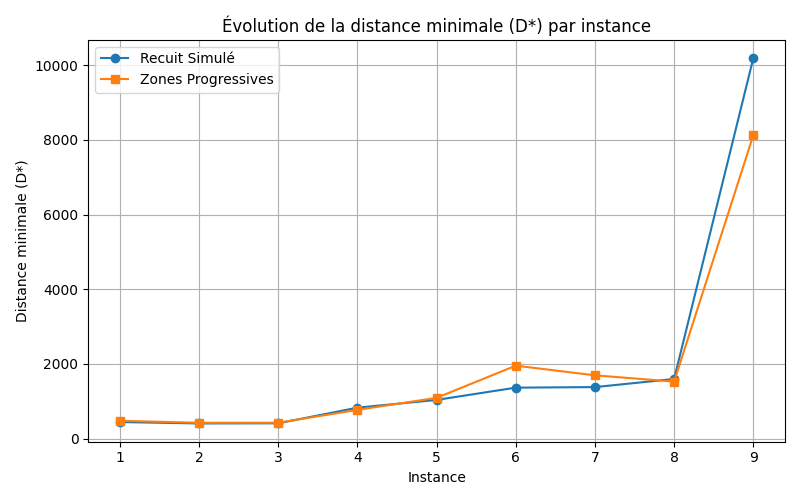
\includegraphics[width=0.7\textwidth]{distance.png}
    \caption{Comparaison des distances totales parcourues entre les deux méthodes}
\end{figure}

\begin{itemize}
    \item \textbf{Déséquilibre global :} Concernant le déséquilibre, l'heuristique de balancement progressif par zones montre une meilleure performance sur certaines instances, atteignant même un déséquilibre nul pour l'instance 6, ce qui indique un équilibrage parfait. Le recuit simulé, bien que performant, présente des déséquilibres plus élevés sur les grandes instances.
\end{itemize}

\begin{figure}[!htbp]
    \centering
    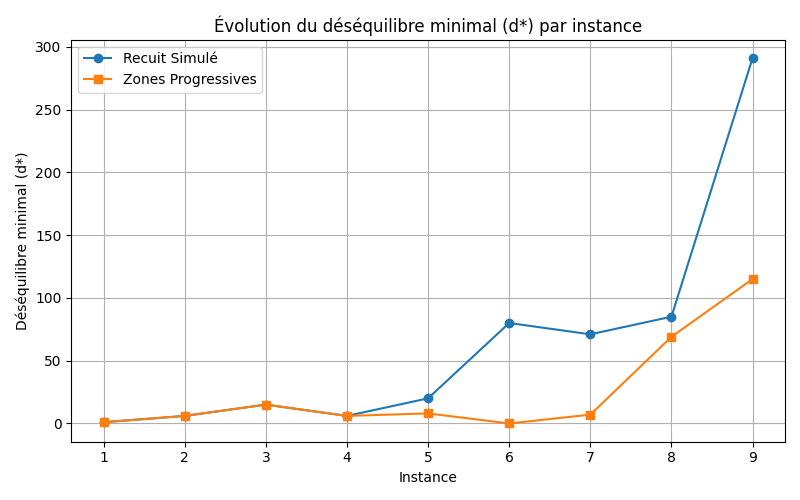
\includegraphics[width=0.7\textwidth]{desequilibre.png}
    \caption{Comparaison du déséquilibre global entre les deux méthodes}
\end{figure}


\vspace{1cm}

\subsection{Récapitulatif Global}

La méthode de recuit simulé offre une meilleure optimisation de la distance totale parcourue, mais au prix d'un temps d'exécution beaucoup plus élevé. L'heuristique de balancement progressif par zones est plus rapide et peut atteindre des déséquilibres plus faibles, voire nuls, sur certaines instances, mais avec des distances parfois plus importantes. Le choix entre ces deux méthodes dépend donc des priorités : précision optimale de la tournée (recuit simulé) ou rapidité et bonne qualité de solution (heuristique).

\section{Conclusion Générale}

Ce rapport a présenté le problème d'équilibrage nocturne d'un parc de vélos en libre-service, ainsi que deux méthodes pour résoudre ce problème : une méthode de recuit simulé lexicographique et une heuristique de balancement progressif par zones.

La modélisation mathématique du problème a été détaillée, suivie de la description des deux approches et de leurs résultats expérimentaux. La comparaison des méthodes a montré que chacune présente des avantages spécifiques : le recuit simulé excelle dans la minimisation de la distance parcourue, tandis que l'heuristique offre un compromis intéressant entre temps de calcul et qualité du déséquilibre.

Ces travaux ouvrent la voie à des améliorations futures, notamment l'intégration de contraintes supplémentaires, l'optimisation des paramètres des algorithmes, et l'adaptation à des contextes urbains variés.

\end{document}